\begin{figure*}[t]
\centering
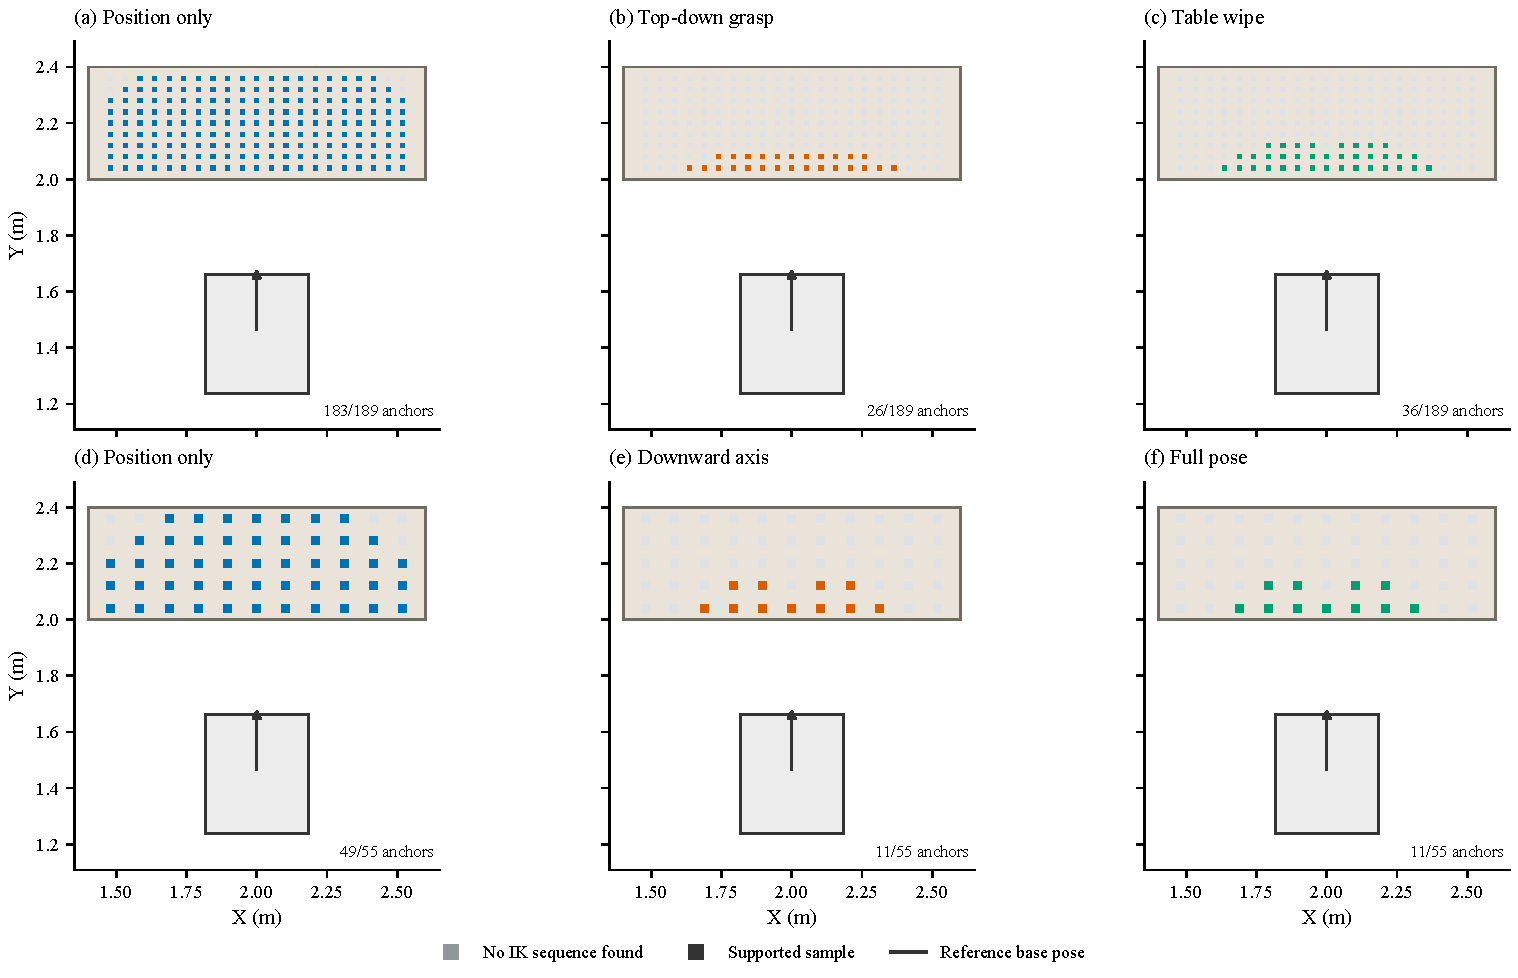
\includegraphics[width=0.98\textwidth]{workspace_support.pdf}
% Full Chinese caption and exact values: workspace_support_caption.md
\caption{Sampled manipulation support under task-specific actions (top row) and matched Cartesian paths (bottom row). Colored samples admit a numerical IK sequence; gray samples denote finite-search failures. All panels share the same world-coordinate limits.}
\label{fig:workspace-support}
\end{figure*}

\begin{figure*}[t]
\centering
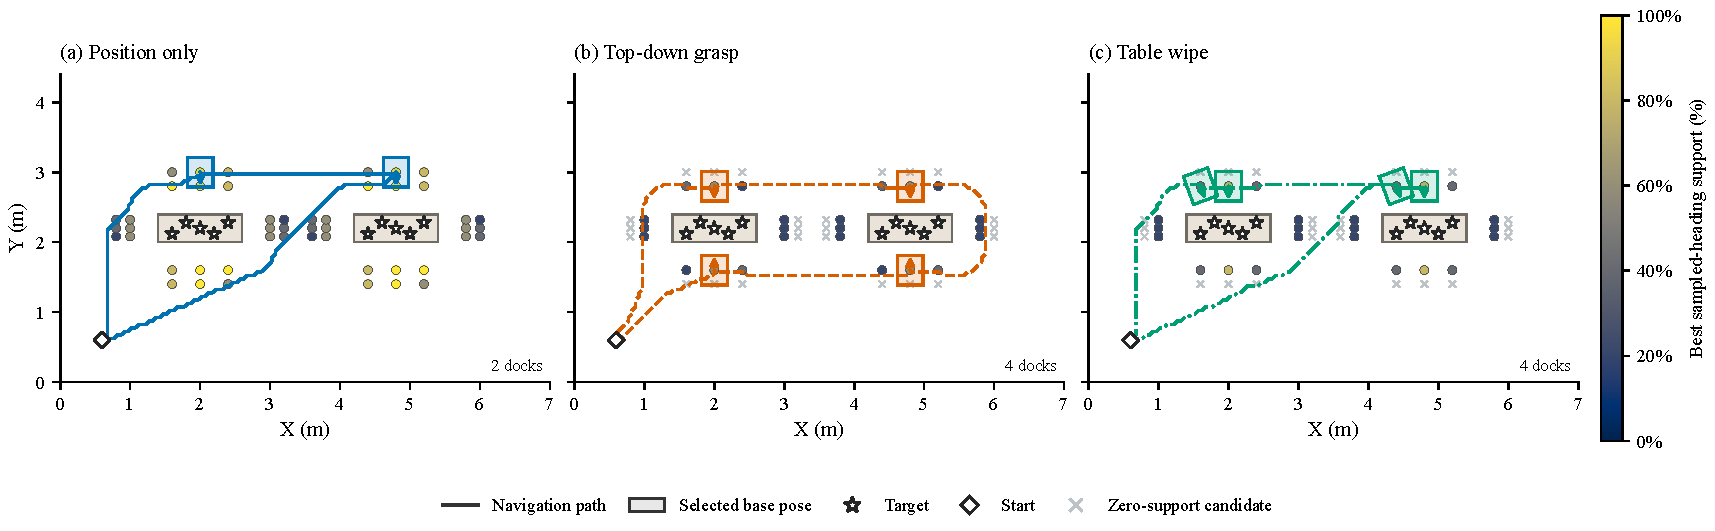
\includegraphics[width=0.98\textwidth]{dock_routes.pdf}
% Full Chinese caption and exact values: dock_routes_caption.md
\caption{Candidate support, selected base poses, and exported navigation paths in the shared scene. Candidate colors show the maximum support ratio over sampled headings at each position. Rectangles and arrows show selected base footprints and orientations.}
\label{fig:dock-routes}
\end{figure*}

\begin{figure*}[t]
\centering
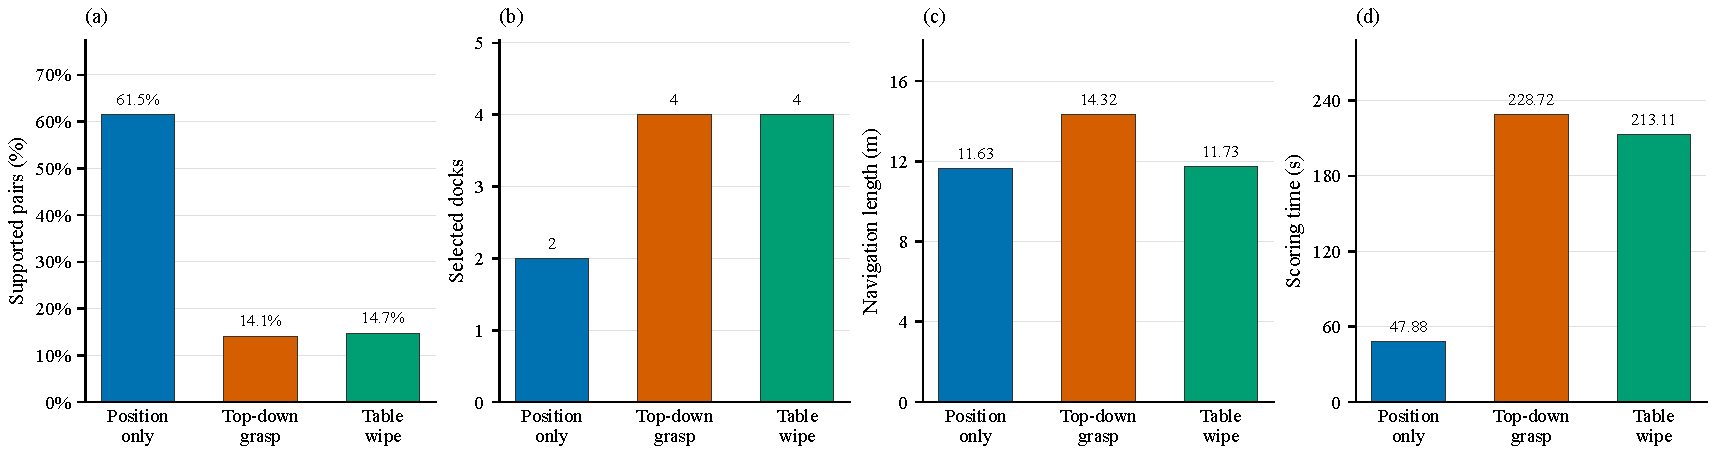
\includegraphics[width=0.98\textwidth]{comparison_metrics.pdf}
% Full Chinese caption and exact values: comparison_metrics_caption.md
\caption{Candidate--target pair support, selected dock counts, navigation length, and observed scoring time. Values describe this exported run; error bars and statistical significance are not inferred. Hatched route bars, if any, denote failed navigation validation.}
\label{fig:comparison-metrics}
\end{figure*}
